\myparagraph{Le nano ordinateur}
\begin{figure}[H]
    \centering
    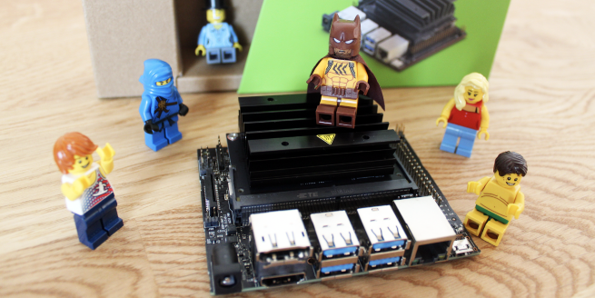
\includegraphics[width=1.0\textwidth]{jetson_nano_lego}
    \caption{Photo de la carte mère Jetson Nano de NVIDIA, représenté avec des Lego pour démontrer sa petitesse}
    \label{fig:jetson_nano_lego}
\end{figure}
\par L'objet d'étude de cet essai est un nano ordinateur. Un nano ordinateur est un ordinateur miniaturisé en taille, mais aussi limité en capacité. Il existe différents fabricants et modèles, de caractéristiques techniques variées, pour répondre à différents besoins. Le dernier né est le modèle "Jetson nano" du fabricant "NVIDIA" (figure \ref{fig:jetson_nano_lego}), disponible depuis juin 2019 au prix très abordable de 99\$US. La compagnie NVIDIA a conçu ce matériel spécialement pour différentes applications d'inférence de modèles d'apprentissage profond sur une plateforme mobile (drone) ou proche des données ("edge" en anglais). Ce modèle a été choisi afin de répondre à l'intérêt que suscitent ses capacités et ses limites. 
\myparagraph{Logiciels}
\par De même que pour les périphériques, les logiciels qui seront utilisés seront résumés dans un tableau, où il sera indiqué leur nom, le type de licence, leur version, leurs avantages et limitations, comme pour le système d'exploitation, l'environnement de développement pour l'apprentissage profond, l'inférence, les logiciels de traitements vidéos et d'images. 
\par Pour tester les performances de la micro-sd et du disque SDD interne M.2 NVMe, l'utilitaire "hdparm" a été utilisé. Il est nécessaire de l'installer (`sudo apt-get install hdparm`) car il n'est pas inclusde base dans le système UBuntu 18.04;
\par Le SDK qui sera utilisé sera celui fourni par NVIDIA et qui se nomme "JetPack". Il contient le système d'exploitation Linux For Tegra (L4T) qui est une version de la distribution Ubuntu 18.04 mise à la saveur de NVIDIA. Jetpack contient aussi d'autres librairies qui sont nécessaires pour l'inférence, tel que Cuda, CuDn et TensorRT.
{\color{red} \par Figure/tableau des versions et description des éléments du framework Jetpack. \todo{TODO}}
\par Le cadre d'application logicielle ("frameworks") d’apprentissage profond qui seront utilisés sont PyTorch avec un fork de torchvision.
{\color{red} \par Figure/tableau des versions, rôle et responsabilité de pytorch et le fork de torchvision dans le cadre de l'essai. \todo{TODO}}
\par Enfin pour régénérer le ONNX, les librairies TensorRT et ONNX a été utilisé, en compagnie de l'utilitaire `tensorrt` qui permet de valider et tester l'ONNX généré.
{\color{red} \par Figure/tableau des versions, rôle et responsabilité de TensorRT, ONNX et tensorrt dans le cadre de l'essai. \todo{TODO}}